\documentclass[10pt, letterpaper, titlepage]{article}

%Size of section header
\usepackage{sectsty}
\sectionfont{\fontsize{12}{15}\selectfont}

%quattrocento font
\usepackage[sfdefault]{quattrocento}

\usepackage{amsmath}
\usepackage{xcolor}
\usepackage{multicol}

%For figures
\usepackage{float}
\floatstyle{boxed} 
\restylefloat{figure}

%Header
\usepackage[margin=1in]{geometry}
\usepackage{fancyhdr}
\setlength{\headheight}{23.01503pt}
\pagestyle{fancy}
\lhead{}
\rhead{Yifeng Pan\\ 
     UCID: 30063828}

%Change lable to letter from number
\renewcommand{\thesubsection}{\alph{subsection}}

%Evaluate for calc
\newcommand*\eval[3]{\left.#1\right\rvert_{#2}^{#3}}

%Absolute Value
\newcommand\abs[1]{\left|#1\right|}

%Title page
\title{STAT 323 Bonus Assignment}
\author{Instructor: Claudia Marie Mahler
    \\Name: Yifeng Pan
    \\UCID: 30063828}
\date{Summer 2019}

\newcommand{\mx}{\overline{x}}
\newcommand{\my}{\overline{y}}
\newcommand{\mz}{\overline{z}}
\newcommand{\mX}{\overline{X}}

%For displaying R code
\usepackage{listings}

%For imported R plots
\usepackage{tikz}

\usepackage{amssymb}
\newcommand{\Z}{\mathbb{Z}}
\newcommand{\R}{\mathbb{R}}

\newcommand{\E}{\text{E}}
\newcommand{\RE}{\text{RE}}
\newcommand{\B}{\text{B}}
\newcommand{\Var}{\text{Var}}
\newcommand{\Cov}{\text{Cov}}
\newcommand{\pv}{\text{p-value}}

\begin{document}
    \maketitle

    \section{Suppose $S \subseteq \R$.}
    \subsection{Show that if $S \neq \R$ and $S \neq \emptyset$, then $\bd(S) \neq \emptyset$.}
        We prove the contrapositive: 
        If $\bd(S) = \emptyset$, then $S = \R$ or $S = \emptyset$.
        Suppose $\bd(S) = \emptyset$.
        If $S = \emptyset$, we are done.
        Let $S \neq \emptyset$. We prove $S = \R$.
        Since $\bd(S) = \emptyset$, $S = \interior(S)$.
        Since $S \neq \emptyset$, let $x_1 \in S$.
        Since $x_1$ is an interior point of $S$,
        $\lis \e_1$ such that $(x_1 - \e_1, x_1 + \e_1) \subseteq S$.
        Let $x_2 = x_1 + \e_1$.
        If $x_2 \not\in S$, then $x_2$ would be a boundary point of $S$,
        which would be a contradiction.
        Therefore $x_2 \in S$.
        We repeat to construct the sequence $\set{x_n}$, and $\set{\e_n}$,
        such that $x_{n+1} > x_n$, 
        and if $x_n < y < x_{n+1}$, then $y \in N_{\e_n}(x_n) \subseteq S$.
        Therefore, $\lall n, [x_1, x_n) \subseteq S$.
        As $n \to \infty$, 
        if $\set{x_n}$ is convergent to $L$, then $L$ is a boundary point of $S$,
        which is a contradiction.
        Therefore $\set{x_n}$ is divergent to infinity, as it's increasing.
        Therefore $[x_1, \infty) \subseteq S$.
        Simularly, we construct the sequence in the negative direction to prove
        $(-\infty, x_1] \subseteq S$.
        Therefore $S = \R$.

    \subsection{Show that $\bd(S) = \overline{S} \intersection \overline{\R \setminus S}$.}
        We know $\bd(S) = \bd(\R \setminus S)$, 
        As they have the same definition.

        % \begin{lemma}
        %     $\bd(S) \subseteq  \overline{S} \intersection \overline{\R \setminus S}$
        % \end{lemma}
            % Proof:
            Suppose $x \in \bd(S)$.
            Since $\bd{S} \subseteq \overline S$,
            $x\in \overline S$.
            Since $x \in \bd(S) = \bd(\R \setminus S)$,
            $x \in \overline{\R \setminus S}$.
            Therefore $x \in \overline{S} \intersection \overline{\R \setminus S}$.
            % \qed

        % \begin{lemma}
        %     $\overline{S} \intersection \overline{\R \setminus S} \subseteq \bd(S)$
        % \end{lemma}
            % Proof:
            Suppose 
            $x \in \overline{S} \intersection \overline{\R \setminus S}
                = (S \union \bd(S)) \intersection ((\R \setminus S \union \bd(\R \setminus S))$.
            Therefore $x \not\in S \lif x \in \bd(S)$
            and $x \in S \lif x \not\in \R \setminus S \lif x \in \bd(\R \setminus S) = \bd(S)$.
            Therefore $x \in \bd(S)$ is both cases.
            % \qed

        Therefore
        $\bd(S) = \overline{S} \intersection \overline{\R \setminus S}$.
    
    \newpage
    %Figures
    \begin{figure}[h]
        \centering
        % Created by tikzDevice version 0.12.3 on 2019-08-18 06:14:08
% !TEX encoding = UTF-8 Unicode
\begin{tikzpicture}[x=1pt,y=1pt]
\definecolor{fillColor}{RGB}{255,255,255}
\path[use as bounding box,fill=fillColor,fill opacity=0.00] (0,0) rectangle (216.81,216.81);
\begin{scope}
\path[clip] (  0.00,  0.00) rectangle (216.81,216.81);
\definecolor{drawColor}{RGB}{0,0,0}

\node[text=drawColor,anchor=base,inner sep=0pt, outer sep=0pt, scale=  1.20] at (120.41,188.07) {\bfseries Histogram of residuals};

\node[text=drawColor,anchor=base,inner sep=0pt, outer sep=0pt, scale=  1.00] at (120.41, 15.60) {Residuals};

\node[text=drawColor,rotate= 90.00,anchor=base,inner sep=0pt, outer sep=0pt, scale=  1.00] at ( 10.80,114.41) {Frequency};
\end{scope}
\begin{scope}
\path[clip] (  0.00,  0.00) rectangle (216.81,216.81);
\definecolor{drawColor}{RGB}{0,0,0}

\path[draw=drawColor,line width= 0.4pt,line join=round,line cap=round] ( 54.47, 61.20) -- (186.34, 61.20);

\path[draw=drawColor,line width= 0.4pt,line join=round,line cap=round] ( 54.47, 61.20) -- ( 54.47, 55.20);

\path[draw=drawColor,line width= 0.4pt,line join=round,line cap=round] ( 80.85, 61.20) -- ( 80.85, 55.20);

\path[draw=drawColor,line width= 0.4pt,line join=round,line cap=round] (107.22, 61.20) -- (107.22, 55.20);

\path[draw=drawColor,line width= 0.4pt,line join=round,line cap=round] (133.59, 61.20) -- (133.59, 55.20);

\path[draw=drawColor,line width= 0.4pt,line join=round,line cap=round] (159.96, 61.20) -- (159.96, 55.20);

\path[draw=drawColor,line width= 0.4pt,line join=round,line cap=round] (186.34, 61.20) -- (186.34, 55.20);

\node[text=drawColor,anchor=base,inner sep=0pt, outer sep=0pt, scale=  1.00] at ( 54.47, 39.60) {-30};

\node[text=drawColor,anchor=base,inner sep=0pt, outer sep=0pt, scale=  1.00] at ( 80.85, 39.60) {-20};

\node[text=drawColor,anchor=base,inner sep=0pt, outer sep=0pt, scale=  1.00] at (107.22, 39.60) {-10};

\node[text=drawColor,anchor=base,inner sep=0pt, outer sep=0pt, scale=  1.00] at (133.59, 39.60) {0};

\node[text=drawColor,anchor=base,inner sep=0pt, outer sep=0pt, scale=  1.00] at (159.96, 39.60) {10};

\node[text=drawColor,anchor=base,inner sep=0pt, outer sep=0pt, scale=  1.00] at (186.34, 39.60) {20};

\path[draw=drawColor,line width= 0.4pt,line join=round,line cap=round] ( 49.20, 65.14) -- ( 49.20,159.88);

\path[draw=drawColor,line width= 0.4pt,line join=round,line cap=round] ( 49.20, 65.14) -- ( 43.20, 65.14);

\path[draw=drawColor,line width= 0.4pt,line join=round,line cap=round] ( 49.20, 84.09) -- ( 43.20, 84.09);

\path[draw=drawColor,line width= 0.4pt,line join=round,line cap=round] ( 49.20,103.04) -- ( 43.20,103.04);

\path[draw=drawColor,line width= 0.4pt,line join=round,line cap=round] ( 49.20,121.98) -- ( 43.20,121.98);

\path[draw=drawColor,line width= 0.4pt,line join=round,line cap=round] ( 49.20,140.93) -- ( 43.20,140.93);

\path[draw=drawColor,line width= 0.4pt,line join=round,line cap=round] ( 49.20,159.88) -- ( 43.20,159.88);

\node[text=drawColor,rotate= 90.00,anchor=base,inner sep=0pt, outer sep=0pt, scale=  1.00] at ( 34.80, 65.14) {0};

\node[text=drawColor,rotate= 90.00,anchor=base,inner sep=0pt, outer sep=0pt, scale=  1.00] at ( 34.80, 84.09) {5};

\node[text=drawColor,rotate= 90.00,anchor=base,inner sep=0pt, outer sep=0pt, scale=  1.00] at ( 34.80,103.04) {10};

\node[text=drawColor,rotate= 90.00,anchor=base,inner sep=0pt, outer sep=0pt, scale=  1.00] at ( 34.80,121.98) {15};

\node[text=drawColor,rotate= 90.00,anchor=base,inner sep=0pt, outer sep=0pt, scale=  1.00] at ( 34.80,140.93) {20};

\node[text=drawColor,rotate= 90.00,anchor=base,inner sep=0pt, outer sep=0pt, scale=  1.00] at ( 34.80,159.88) {25};
\end{scope}
\begin{scope}
\path[clip] ( 49.20, 61.20) rectangle (191.61,167.61);
\definecolor{drawColor}{RGB}{0,0,0}

\path[draw=drawColor,line width= 0.4pt,line join=round,line cap=round] ( 54.47, 65.14) rectangle ( 67.66, 72.72);

\path[draw=drawColor,line width= 0.4pt,line join=round,line cap=round] ( 67.66, 65.14) rectangle ( 80.85, 72.72);

\path[draw=drawColor,line width= 0.4pt,line join=round,line cap=round] ( 80.85, 65.14) rectangle ( 94.03, 84.09);

\path[draw=drawColor,line width= 0.4pt,line join=round,line cap=round] ( 94.03, 65.14) rectangle (107.22, 99.25);

\path[draw=drawColor,line width= 0.4pt,line join=round,line cap=round] (107.22, 65.14) rectangle (120.41,114.40);

\path[draw=drawColor,line width= 0.4pt,line join=round,line cap=round] (120.41, 65.14) rectangle (133.59,144.72);

\path[draw=drawColor,line width= 0.4pt,line join=round,line cap=round] (133.59, 65.14) rectangle (146.78,152.30);

\path[draw=drawColor,line width= 0.4pt,line join=round,line cap=round] (146.78, 65.14) rectangle (159.96,163.67);

\path[draw=drawColor,line width= 0.4pt,line join=round,line cap=round] (159.96, 65.14) rectangle (173.15, 95.46);

\path[draw=drawColor,line width= 0.4pt,line join=round,line cap=round] (173.15, 65.14) rectangle (186.34, 76.51);
\end{scope}
\end{tikzpicture}
\begin{tikzpicture}[x=1pt,y=1pt]
\definecolor{fillColor}{RGB}{255,255,255}
\path[use as bounding box,fill=fillColor,fill opacity=0.00] (0,0) rectangle (216.81,216.81);
\begin{scope}
\path[clip] ( 49.20, 61.20) rectangle (191.61,167.61);
\definecolor{drawColor}{RGB}{0,0,0}

\path[draw=drawColor,line width= 0.4pt,line join=round,line cap=round] (113.84,118.32) circle (  2.25);

\path[draw=drawColor,line width= 0.4pt,line join=round,line cap=round] (129.34,130.36) circle (  2.25);

\path[draw=drawColor,line width= 0.4pt,line join=round,line cap=round] (102.32,109.30) circle (  2.25);

\path[draw=drawColor,line width= 0.4pt,line join=round,line cap=round] (118.43,121.25) circle (  2.25);

\path[draw=drawColor,line width= 0.4pt,line join=round,line cap=round] (124.66,126.58) circle (  2.25);

\path[draw=drawColor,line width= 0.4pt,line join=round,line cap=round] ( 99.26,105.03) circle (  2.25);

\path[draw=drawColor,line width= 0.4pt,line join=round,line cap=round] (158.20,145.58) circle (  2.25);

\path[draw=drawColor,line width= 0.4pt,line join=round,line cap=round] (176.25,153.55) circle (  2.25);

\path[draw=drawColor,line width= 0.4pt,line join=round,line cap=round] (135.68,136.12) circle (  2.25);

\path[draw=drawColor,line width= 0.4pt,line join=round,line cap=round] (100.83,108.32) circle (  2.25);

\path[draw=drawColor,line width= 0.4pt,line join=round,line cap=round] ( 85.78, 92.87) circle (  2.25);

\path[draw=drawColor,line width= 0.4pt,line join=round,line cap=round] (105.80,111.80) circle (  2.25);

\path[draw=drawColor,line width= 0.4pt,line join=round,line cap=round] (125.23,126.58) circle (  2.25);

\path[draw=drawColor,line width= 0.4pt,line join=round,line cap=round] (114.42,118.66) circle (  2.25);

\path[draw=drawColor,line width= 0.4pt,line join=round,line cap=round] (167.37,149.10) circle (  2.25);

\path[draw=drawColor,line width= 0.4pt,line join=round,line cap=round] (148.87,140.43) circle (  2.25);

\path[draw=drawColor,line width= 0.4pt,line join=round,line cap=round] (108.40,113.96) circle (  2.25);

\path[draw=drawColor,line width= 0.4pt,line join=round,line cap=round] (153.64,140.81) circle (  2.25);

\path[draw=drawColor,line width= 0.4pt,line join=round,line cap=round] ( 69.77, 72.99) circle (  2.25);

\path[draw=drawColor,line width= 0.4pt,line join=round,line cap=round] (133.05,133.10) circle (  2.25);

\path[draw=drawColor,line width= 0.4pt,line join=round,line cap=round] ( 73.44, 76.83) circle (  2.25);

\path[draw=drawColor,line width= 0.4pt,line join=round,line cap=round] (121.82,123.84) circle (  2.25);

\path[draw=drawColor,line width= 0.4pt,line join=round,line cap=round] ( 84.27, 90.43) circle (  2.25);

\path[draw=drawColor,line width= 0.4pt,line join=round,line cap=round] (119.56,121.87) circle (  2.25);

\path[draw=drawColor,line width= 0.4pt,line join=round,line cap=round] (120.69,122.83) circle (  2.25);

\path[draw=drawColor,line width= 0.4pt,line join=round,line cap=round] (138.49,136.15) circle (  2.25);

\path[draw=drawColor,line width= 0.4pt,line join=round,line cap=round] ( 93.98,100.85) circle (  2.25);

\path[draw=drawColor,line width= 0.4pt,line join=round,line cap=round] (117.86,120.50) circle (  2.25);

\path[draw=drawColor,line width= 0.4pt,line join=round,line cap=round] ( 91.94, 98.64) circle (  2.25);

\path[draw=drawColor,line width= 0.4pt,line join=round,line cap=round] (116.72,120.23) circle (  2.25);

\path[draw=drawColor,line width= 0.4pt,line join=round,line cap=round] ( 97.61,103.06) circle (  2.25);

\path[draw=drawColor,line width= 0.4pt,line join=round,line cap=round] (112.07,117.11) circle (  2.25);

\path[draw=drawColor,line width= 0.4pt,line join=round,line cap=round] (121.25,123.23) circle (  2.25);

\path[draw=drawColor,line width= 0.4pt,line join=round,line cap=round] (103.75,109.82) circle (  2.25);

\path[draw=drawColor,line width= 0.4pt,line join=round,line cap=round] (129.94,130.36) circle (  2.25);

\path[draw=drawColor,line width= 0.4pt,line join=round,line cap=round] (123.52,125.01) circle (  2.25);

\path[draw=drawColor,line width= 0.4pt,line join=round,line cap=round] (133.69,134.32) circle (  2.25);

\path[draw=drawColor,line width= 0.4pt,line join=round,line cap=round] (132.41,130.93) circle (  2.25);

\path[draw=drawColor,line width= 0.4pt,line join=round,line cap=round] (116.15,120.10) circle (  2.25);

\path[draw=drawColor,line width= 0.4pt,line join=round,line cap=round] (156.54,145.37) circle (  2.25);

\path[draw=drawColor,line width= 0.4pt,line join=round,line cap=round] (136.36,136.12) circle (  2.25);

\path[draw=drawColor,line width= 0.4pt,line join=round,line cap=round] (130.55,130.36) circle (  2.25);

\path[draw=drawColor,line width= 0.4pt,line join=round,line cap=round] ( 78.71, 88.97) circle (  2.25);

\path[draw=drawColor,line width= 0.4pt,line join=round,line cap=round] (115.00,119.49) circle (  2.25);

\path[draw=drawColor,line width= 0.4pt,line join=round,line cap=round] (160.03,145.58) circle (  2.25);

\path[draw=drawColor,line width= 0.4pt,line join=round,line cap=round] (110.26,116.26) circle (  2.25);

\path[draw=drawColor,line width= 0.4pt,line join=round,line cap=round] (127.55,128.56) circle (  2.25);

\path[draw=drawColor,line width= 0.4pt,line join=round,line cap=round] (131.16,130.36) circle (  2.25);

\path[draw=drawColor,line width= 0.4pt,line join=round,line cap=round] (142.36,137.26) circle (  2.25);

\path[draw=drawColor,line width= 0.4pt,line join=round,line cap=round] (111.47,116.68) circle (  2.25);

\path[draw=drawColor,line width= 0.4pt,line join=round,line cap=round] (143.20,137.67) circle (  2.25);

\path[draw=drawColor,line width= 0.4pt,line join=round,line cap=round] (107.76,112.94) circle (  2.25);

\path[draw=drawColor,line width= 0.4pt,line join=round,line cap=round] ( 80.78, 89.03) circle (  2.25);

\path[draw=drawColor,line width= 0.4pt,line join=round,line cap=round] ( 89.69, 96.18) circle (  2.25);

\path[draw=drawColor,line width= 0.4pt,line join=round,line cap=round] (128.74,130.16) circle (  2.25);

\path[draw=drawColor,line width= 0.4pt,line join=round,line cap=round] (106.46,112.56) circle (  2.25);

\path[draw=drawColor,line width= 0.4pt,line join=round,line cap=round] ( 92.98, 98.87) circle (  2.25);

\path[draw=drawColor,line width= 0.4pt,line join=round,line cap=round] (164.50,146.92) circle (  2.25);

\path[draw=drawColor,line width= 0.4pt,line join=round,line cap=round] (101.58,108.76) circle (  2.25);

\path[draw=drawColor,line width= 0.4pt,line join=round,line cap=round] (149.96,140.43) circle (  2.25);

\path[draw=drawColor,line width= 0.4pt,line join=round,line cap=round] (131.78,130.73) circle (  2.25);

\path[draw=drawColor,line width= 0.4pt,line join=round,line cap=round] (139.23,136.47) circle (  2.25);

\path[draw=drawColor,line width= 0.4pt,line join=round,line cap=round] (126.97,127.58) circle (  2.25);

\path[draw=drawColor,line width= 0.4pt,line join=round,line cap=round] (110.87,116.26) circle (  2.25);

\path[draw=drawColor,line width= 0.4pt,line join=round,line cap=round] (112.67,117.11) circle (  2.25);

\path[draw=drawColor,line width= 0.4pt,line join=round,line cap=round] (100.06,106.79) circle (  2.25);

\path[draw=drawColor,line width= 0.4pt,line join=round,line cap=round] (144.95,139.44) circle (  2.25);

\path[draw=drawColor,line width= 0.4pt,line join=round,line cap=round] ( 54.47, 65.14) circle (  2.25);

\path[draw=drawColor,line width= 0.4pt,line join=round,line cap=round] (107.12,112.72) circle (  2.25);

\path[draw=drawColor,line width= 0.4pt,line join=round,line cap=round] ( 64.56, 69.18) circle (  2.25);

\path[draw=drawColor,line width= 0.4pt,line join=round,line cap=round] (117.29,120.23) circle (  2.25);

\path[draw=drawColor,line width= 0.4pt,line join=round,line cap=round] (145.87,139.44) circle (  2.25);

\path[draw=drawColor,line width= 0.4pt,line join=round,line cap=round] (151.12,140.43) circle (  2.25);

\path[draw=drawColor,line width= 0.4pt,line join=round,line cap=round] (137.06,136.12) circle (  2.25);

\path[draw=drawColor,line width= 0.4pt,line join=round,line cap=round] (109.65,115.74) circle (  2.25);

\path[draw=drawColor,line width= 0.4pt,line join=round,line cap=round] (113.26,118.25) circle (  2.25);

\path[draw=drawColor,line width= 0.4pt,line join=round,line cap=round] ( 82.61, 89.03) circle (  2.25);

\path[draw=drawColor,line width= 0.4pt,line join=round,line cap=round] (128.14,128.96) circle (  2.25);

\path[draw=drawColor,line width= 0.4pt,line join=round,line cap=round] (122.95,124.60) circle (  2.25);

\path[draw=drawColor,line width= 0.4pt,line join=round,line cap=round] (171.04,152.05) circle (  2.25);

\path[draw=drawColor,line width= 0.4pt,line join=round,line cap=round] (146.83,139.44) circle (  2.25);

\path[draw=drawColor,line width= 0.4pt,line join=round,line cap=round] ( 95.86,101.54) circle (  2.25);

\path[draw=drawColor,line width= 0.4pt,line join=round,line cap=round] ( 94.94,100.85) circle (  2.25);

\path[draw=drawColor,line width= 0.4pt,line join=round,line cap=round] (140.75,136.86) circle (  2.25);

\path[draw=drawColor,line width= 0.4pt,line join=round,line cap=round] ( 90.85, 96.89) circle (  2.25);

\path[draw=drawColor,line width= 0.4pt,line join=round,line cap=round] (139.98,136.66) circle (  2.25);

\path[draw=drawColor,line width= 0.4pt,line join=round,line cap=round] ( 88.47, 94.67) circle (  2.25);

\path[draw=drawColor,line width= 0.4pt,line join=round,line cap=round] (144.06,138.86) circle (  2.25);

\path[draw=drawColor,line width= 0.4pt,line join=round,line cap=round] ( 87.17, 93.82) circle (  2.25);

\path[draw=drawColor,line width= 0.4pt,line join=round,line cap=round] (120.12,122.62) circle (  2.25);

\path[draw=drawColor,line width= 0.4pt,line join=round,line cap=round] (135.01,135.89) circle (  2.25);

\path[draw=drawColor,line width= 0.4pt,line join=round,line cap=round] (125.81,126.78) circle (  2.25);

\path[draw=drawColor,line width= 0.4pt,line join=round,line cap=round] (104.45,110.40) circle (  2.25);

\path[draw=drawColor,line width= 0.4pt,line join=round,line cap=round] ( 96.75,101.72) circle (  2.25);

\path[draw=drawColor,line width= 0.4pt,line join=round,line cap=round] (152.34,140.43) circle (  2.25);

\path[draw=drawColor,line width= 0.4pt,line join=round,line cap=round] ( 98.45,104.46) circle (  2.25);

\path[draw=drawColor,line width= 0.4pt,line join=round,line cap=round] (137.77,136.12) circle (  2.25);

\path[draw=drawColor,line width= 0.4pt,line join=round,line cap=round] (147.83,140.11) circle (  2.25);

\path[draw=drawColor,line width= 0.4pt,line join=round,line cap=round] (186.34,156.79) circle (  2.25);

\path[draw=drawColor,line width= 0.4pt,line join=round,line cap=round] (141.55,136.86) circle (  2.25);

\path[draw=drawColor,line width= 0.4pt,line join=round,line cap=round] (105.13,110.58) circle (  2.25);

\path[draw=drawColor,line width= 0.4pt,line join=round,line cap=round] (155.03,144.76) circle (  2.25);

\path[draw=drawColor,line width= 0.4pt,line join=round,line cap=round] (126.39,127.18) circle (  2.25);

\path[draw=drawColor,line width= 0.4pt,line join=round,line cap=round] (109.03,115.13) circle (  2.25);

\path[draw=drawColor,line width= 0.4pt,line join=round,line cap=round] (118.99,121.33) circle (  2.25);

\path[draw=drawColor,line width= 0.4pt,line join=round,line cap=round] (162.10,146.32) circle (  2.25);

\path[draw=drawColor,line width= 0.4pt,line join=round,line cap=round] (122.38,124.05) circle (  2.25);

\path[draw=drawColor,line width= 0.4pt,line join=round,line cap=round] (115.58,119.94) circle (  2.25);

\path[draw=drawColor,line width= 0.4pt,line join=round,line cap=round] (103.04,109.41) circle (  2.25);

\path[draw=drawColor,line width= 0.4pt,line join=round,line cap=round] (124.09,125.01) circle (  2.25);

\path[draw=drawColor,line width= 0.4pt,line join=round,line cap=round] ( 76.31, 83.29) circle (  2.25);

\path[draw=drawColor,line width= 0.4pt,line join=round,line cap=round] (134.35,134.69) circle (  2.25);
\end{scope}
\begin{scope}
\path[clip] (  0.00,  0.00) rectangle (216.81,216.81);
\definecolor{drawColor}{RGB}{0,0,0}

\path[draw=drawColor,line width= 0.4pt,line join=round,line cap=round] ( 69.98, 61.20) -- (170.83, 61.20);

\path[draw=drawColor,line width= 0.4pt,line join=round,line cap=round] ( 69.98, 61.20) -- ( 69.98, 55.20);

\path[draw=drawColor,line width= 0.4pt,line join=round,line cap=round] ( 95.19, 61.20) -- ( 95.19, 55.20);

\path[draw=drawColor,line width= 0.4pt,line join=round,line cap=round] (120.40, 61.20) -- (120.40, 55.20);

\path[draw=drawColor,line width= 0.4pt,line join=round,line cap=round] (145.62, 61.20) -- (145.62, 55.20);

\path[draw=drawColor,line width= 0.4pt,line join=round,line cap=round] (170.83, 61.20) -- (170.83, 55.20);

\node[text=drawColor,anchor=base,inner sep=0pt, outer sep=0pt, scale=  1.00] at ( 69.98, 39.60) {-2};

\node[text=drawColor,anchor=base,inner sep=0pt, outer sep=0pt, scale=  1.00] at ( 95.19, 39.60) {-1};

\node[text=drawColor,anchor=base,inner sep=0pt, outer sep=0pt, scale=  1.00] at (120.40, 39.60) {0};

\node[text=drawColor,anchor=base,inner sep=0pt, outer sep=0pt, scale=  1.00] at (145.62, 39.60) {1};

\node[text=drawColor,anchor=base,inner sep=0pt, outer sep=0pt, scale=  1.00] at (170.83, 39.60) {2};

\path[draw=drawColor,line width= 0.4pt,line join=round,line cap=round] ( 49.20, 64.44) -- ( 49.20,158.36);

\path[draw=drawColor,line width= 0.4pt,line join=round,line cap=round] ( 49.20, 64.44) -- ( 43.20, 64.44);

\path[draw=drawColor,line width= 0.4pt,line join=round,line cap=round] ( 49.20, 83.23) -- ( 43.20, 83.23);

\path[draw=drawColor,line width= 0.4pt,line join=round,line cap=round] ( 49.20,102.01) -- ( 43.20,102.01);

\path[draw=drawColor,line width= 0.4pt,line join=round,line cap=round] ( 49.20,120.79) -- ( 43.20,120.79);

\path[draw=drawColor,line width= 0.4pt,line join=round,line cap=round] ( 49.20,139.58) -- ( 43.20,139.58);

\path[draw=drawColor,line width= 0.4pt,line join=round,line cap=round] ( 49.20,158.36) -- ( 43.20,158.36);

\node[text=drawColor,rotate= 90.00,anchor=base,inner sep=0pt, outer sep=0pt, scale=  1.00] at ( 34.80, 64.44) {-3};

\node[text=drawColor,rotate= 90.00,anchor=base,inner sep=0pt, outer sep=0pt, scale=  1.00] at ( 34.80, 83.23) {-2};

\node[text=drawColor,rotate= 90.00,anchor=base,inner sep=0pt, outer sep=0pt, scale=  1.00] at ( 34.80,102.01) {-1};

\node[text=drawColor,rotate= 90.00,anchor=base,inner sep=0pt, outer sep=0pt, scale=  1.00] at ( 34.80,120.79) {0};

\node[text=drawColor,rotate= 90.00,anchor=base,inner sep=0pt, outer sep=0pt, scale=  1.00] at ( 34.80,139.58) {1};

\node[text=drawColor,rotate= 90.00,anchor=base,inner sep=0pt, outer sep=0pt, scale=  1.00] at ( 34.80,158.36) {2};

\path[draw=drawColor,line width= 0.4pt,line join=round,line cap=round] ( 49.20, 61.20) --
	(191.61, 61.20) --
	(191.61,167.61) --
	( 49.20,167.61) --
	( 49.20, 61.20);
\end{scope}
\begin{scope}
\path[clip] (  0.00,  0.00) rectangle (216.81,216.81);
\definecolor{drawColor}{RGB}{0,0,0}

\node[text=drawColor,anchor=base,inner sep=0pt, outer sep=0pt, scale=  1.00] at (120.41, 15.60) {Theoretical Quantiles};

\node[text=drawColor,rotate= 90.00,anchor=base,inner sep=0pt, outer sep=0pt, scale=  1.00] at ( 10.80,114.41) {Standardized residuals};
\end{scope}
\begin{scope}
\path[clip] ( 49.20, 61.20) rectangle (191.61,167.61);
\definecolor{drawColor}{gray}{0.50}

\path[draw=drawColor,line width= 0.4pt,dash pattern=on 1pt off 3pt ,line join=round,line cap=round] ( 49.20, 67.64) -- (191.61,178.20);
\end{scope}
\begin{scope}
\path[clip] (  0.00,  0.00) rectangle (216.81,216.81);
\definecolor{drawColor}{RGB}{0,0,0}

\node[text=drawColor,anchor=base,inner sep=0pt, outer sep=0pt, scale=  1.00] at (120.41,  3.60) {lm(Midterm2 ~ Midterm1)};
\end{scope}
\begin{scope}
\path[clip] (  0.00,  0.00) rectangle (216.81,216.81);
\definecolor{drawColor}{RGB}{0,0,0}

\node[text=drawColor,anchor=base,inner sep=0pt, outer sep=0pt, scale=  1.00] at (120.41,173.01) {Normal Q-Q};
\end{scope}
\begin{scope}
\path[clip] (  0.00,  0.00) rectangle (216.81,216.81);
\definecolor{drawColor}{RGB}{0,0,0}

\node[text=drawColor,anchor=base west,inner sep=0pt, outer sep=0pt, scale=  0.75] at ( 57.47, 63.42) {68};

\node[text=drawColor,anchor=base east,inner sep=0pt, outer sep=0pt, scale=  0.75] at ( 61.56, 67.46) {70};

\node[text=drawColor,anchor=base east,inner sep=0pt, outer sep=0pt, scale=  0.75] at ( 66.77, 71.27) {19};
\end{scope}
\end{tikzpicture}

        \caption{}
        \label{fig:1h}
    \end{figure}
    \begin{figure}[h]
        \centering
        % Created by tikzDevice version 0.12.3 on 2019-08-18 20:45:55
% !TEX encoding = UTF-8 Unicode
\begin{tikzpicture}[x=1pt,y=1pt]
\definecolor{fillColor}{RGB}{255,255,255}
\path[use as bounding box,fill=fillColor,fill opacity=0.00] (0,0) rectangle (216.81,216.81);
\begin{scope}
\path[clip] (  0.00,  0.00) rectangle (216.81,216.81);
\definecolor{drawColor}{RGB}{0,0,0}

\node[text=drawColor,anchor=base,inner sep=0pt, outer sep=0pt, scale=  1.20] at (120.41,188.07) {\bfseries Histogram of residuals};

\node[text=drawColor,anchor=base,inner sep=0pt, outer sep=0pt, scale=  1.00] at (120.41, 15.60) {Residuals};

\node[text=drawColor,rotate= 90.00,anchor=base,inner sep=0pt, outer sep=0pt, scale=  1.00] at ( 10.80,114.41) {Frequency};
\end{scope}
\begin{scope}
\path[clip] (  0.00,  0.00) rectangle (216.81,216.81);
\definecolor{drawColor}{RGB}{0,0,0}

\path[draw=drawColor,line width= 0.4pt,line join=round,line cap=round] ( 54.47, 61.20) -- (186.34, 61.20);

\path[draw=drawColor,line width= 0.4pt,line join=round,line cap=round] ( 54.47, 61.20) -- ( 54.47, 55.20);

\path[draw=drawColor,line width= 0.4pt,line join=round,line cap=round] ( 80.85, 61.20) -- ( 80.85, 55.20);

\path[draw=drawColor,line width= 0.4pt,line join=round,line cap=round] (107.22, 61.20) -- (107.22, 55.20);

\path[draw=drawColor,line width= 0.4pt,line join=round,line cap=round] (133.59, 61.20) -- (133.59, 55.20);

\path[draw=drawColor,line width= 0.4pt,line join=round,line cap=round] (159.96, 61.20) -- (159.96, 55.20);

\path[draw=drawColor,line width= 0.4pt,line join=round,line cap=round] (186.34, 61.20) -- (186.34, 55.20);

\node[text=drawColor,anchor=base,inner sep=0pt, outer sep=0pt, scale=  1.00] at ( 54.47, 39.60) {-10000};

\node[text=drawColor,anchor=base,inner sep=0pt, outer sep=0pt, scale=  1.00] at (107.22, 39.60) {0};

\node[text=drawColor,anchor=base,inner sep=0pt, outer sep=0pt, scale=  1.00] at (133.59, 39.60) {5000};

\node[text=drawColor,anchor=base,inner sep=0pt, outer sep=0pt, scale=  1.00] at (186.34, 39.60) {15000};

\path[draw=drawColor,line width= 0.4pt,line join=round,line cap=round] ( 49.20, 65.14) -- ( 49.20,150.82);

\path[draw=drawColor,line width= 0.4pt,line join=round,line cap=round] ( 49.20, 65.14) -- ( 43.20, 65.14);

\path[draw=drawColor,line width= 0.4pt,line join=round,line cap=round] ( 49.20, 86.56) -- ( 43.20, 86.56);

\path[draw=drawColor,line width= 0.4pt,line join=round,line cap=round] ( 49.20,107.98) -- ( 43.20,107.98);

\path[draw=drawColor,line width= 0.4pt,line join=round,line cap=round] ( 49.20,129.40) -- ( 43.20,129.40);

\path[draw=drawColor,line width= 0.4pt,line join=round,line cap=round] ( 49.20,150.82) -- ( 43.20,150.82);

\node[text=drawColor,rotate= 90.00,anchor=base,inner sep=0pt, outer sep=0pt, scale=  1.00] at ( 34.80, 65.14) {0};

\node[text=drawColor,rotate= 90.00,anchor=base,inner sep=0pt, outer sep=0pt, scale=  1.00] at ( 34.80, 86.56) {5};

\node[text=drawColor,rotate= 90.00,anchor=base,inner sep=0pt, outer sep=0pt, scale=  1.00] at ( 34.80,107.98) {10};

\node[text=drawColor,rotate= 90.00,anchor=base,inner sep=0pt, outer sep=0pt, scale=  1.00] at ( 34.80,129.40) {15};

\node[text=drawColor,rotate= 90.00,anchor=base,inner sep=0pt, outer sep=0pt, scale=  1.00] at ( 34.80,150.82) {20};
\end{scope}
\begin{scope}
\path[clip] ( 49.20, 61.20) rectangle (191.61,167.61);
\definecolor{drawColor}{RGB}{0,0,0}

\path[draw=drawColor,line width= 0.4pt,line join=round,line cap=round] ( 54.47, 65.14) rectangle ( 80.85, 90.84);

\path[draw=drawColor,line width= 0.4pt,line join=round,line cap=round] ( 80.85, 65.14) rectangle (107.22,163.67);

\path[draw=drawColor,line width= 0.4pt,line join=round,line cap=round] (107.22, 65.14) rectangle (133.59,129.40);

\path[draw=drawColor,line width= 0.4pt,line join=round,line cap=round] (133.59, 65.14) rectangle (159.96, 95.13);

\path[draw=drawColor,line width= 0.4pt,line join=round,line cap=round] (159.96, 65.14) rectangle (186.34, 69.42);
\end{scope}
\end{tikzpicture}
\begin{tikzpicture}[x=1pt,y=1pt]
\definecolor{fillColor}{RGB}{255,255,255}
\path[use as bounding box,fill=fillColor,fill opacity=0.00] (0,0) rectangle (216.81,216.81);
\begin{scope}
\path[clip] ( 49.20, 61.20) rectangle (191.61,167.61);
\definecolor{drawColor}{RGB}{0,0,0}

\path[draw=drawColor,line width= 0.4pt,line join=round,line cap=round] (150.30,131.42) circle (  2.25);

\path[draw=drawColor,line width= 0.4pt,line join=round,line cap=round] (173.86,148.37) circle (  2.25);

\path[draw=drawColor,line width= 0.4pt,line join=round,line cap=round] (130.82,115.69) circle (  2.25);

\path[draw=drawColor,line width= 0.4pt,line join=round,line cap=round] (112.85,102.69) circle (  2.25);

\path[draw=drawColor,line width= 0.4pt,line join=round,line cap=round] (148.01,127.96) circle (  2.25);

\path[draw=drawColor,line width= 0.4pt,line join=round,line cap=round] (142.04,120.43) circle (  2.25);

\path[draw=drawColor,line width= 0.4pt,line join=round,line cap=round] ( 85.22, 85.66) circle (  2.25);

\path[draw=drawColor,line width= 0.4pt,line join=round,line cap=round] (167.26,140.13) circle (  2.25);

\path[draw=drawColor,line width= 0.4pt,line join=round,line cap=round] (140.26,119.83) circle (  2.25);

\path[draw=drawColor,line width= 0.4pt,line join=round,line cap=round] (143.91,122.55) circle (  2.25);

\path[draw=drawColor,line width= 0.4pt,line join=round,line cap=round] (129.38,112.28) circle (  2.25);

\path[draw=drawColor,line width= 0.4pt,line join=round,line cap=round] (122.44,107.50) circle (  2.25);

\path[draw=drawColor,line width= 0.4pt,line join=round,line cap=round] (145.90,125.79) circle (  2.25);

\path[draw=drawColor,line width= 0.4pt,line join=round,line cap=round] ( 90.51, 89.30) circle (  2.25);

\path[draw=drawColor,line width= 0.4pt,line join=round,line cap=round] (117.00,103.35) circle (  2.25);

\path[draw=drawColor,line width= 0.4pt,line join=round,line cap=round] (158.77,134.10) circle (  2.25);

\path[draw=drawColor,line width= 0.4pt,line join=round,line cap=round] (155.59,133.35) circle (  2.25);

\path[draw=drawColor,line width= 0.4pt,line join=round,line cap=round] (133.79,115.91) circle (  2.25);

\path[draw=drawColor,line width= 0.4pt,line join=round,line cap=round] (119.73,106.29) circle (  2.25);

\path[draw=drawColor,line width= 0.4pt,line join=round,line cap=round] (114.25,102.82) circle (  2.25);

\path[draw=drawColor,line width= 0.4pt,line join=round,line cap=round] ( 73.55, 76.52) circle (  2.25);

\path[draw=drawColor,line width= 0.4pt,line join=round,line cap=round] ( 66.95, 68.14) circle (  2.25);

\path[draw=drawColor,line width= 0.4pt,line join=round,line cap=round] (152.80,131.52) circle (  2.25);

\path[draw=drawColor,line width= 0.4pt,line join=round,line cap=round] (186.34,156.79) circle (  2.25);

\path[draw=drawColor,line width= 0.4pt,line join=round,line cap=round] (138.56,119.69) circle (  2.25);

\path[draw=drawColor,line width= 0.4pt,line join=round,line cap=round] (127.96,112.00) circle (  2.25);

\path[draw=drawColor,line width= 0.4pt,line join=round,line cap=round] (135.33,116.16) circle (  2.25);

\path[draw=drawColor,line width= 0.4pt,line join=round,line cap=round] (132.29,115.81) circle (  2.25);

\path[draw=drawColor,line width= 0.4pt,line join=round,line cap=round] (162.54,134.15) circle (  2.25);

\path[draw=drawColor,line width= 0.4pt,line join=round,line cap=round] (121.08,106.45) circle (  2.25);

\path[draw=drawColor,line width= 0.4pt,line join=round,line cap=round] (107.02,100.64) circle (  2.25);

\path[draw=drawColor,line width= 0.4pt,line join=round,line cap=round] ( 82.04, 80.39) circle (  2.25);

\path[draw=drawColor,line width= 0.4pt,line join=round,line cap=round] (125.18,111.46) circle (  2.25);

\path[draw=drawColor,line width= 0.4pt,line join=round,line cap=round] ( 54.47, 65.14) circle (  2.25);

\path[draw=drawColor,line width= 0.4pt,line join=round,line cap=round] ( 78.27, 80.24) circle (  2.25);

\path[draw=drawColor,line width= 0.4pt,line join=round,line cap=round] (123.81,107.53) circle (  2.25);

\path[draw=drawColor,line width= 0.4pt,line join=round,line cap=round] ( 88.01, 88.08) circle (  2.25);

\path[draw=drawColor,line width= 0.4pt,line join=round,line cap=round] (103.89, 99.62) circle (  2.25);

\path[draw=drawColor,line width= 0.4pt,line join=round,line cap=round] (100.55, 96.21) circle (  2.25);

\path[draw=drawColor,line width= 0.4pt,line join=round,line cap=round] (109.99,101.84) circle (  2.25);

\path[draw=drawColor,line width= 0.4pt,line join=round,line cap=round] (118.37,103.92) circle (  2.25);

\path[draw=drawColor,line width= 0.4pt,line join=round,line cap=round] ( 92.80, 91.80) circle (  2.25);

\path[draw=drawColor,line width= 0.4pt,line join=round,line cap=round] (126.56,111.58) circle (  2.25);

\path[draw=drawColor,line width= 0.4pt,line join=round,line cap=round] (111.43,102.00) circle (  2.25);

\path[draw=drawColor,line width= 0.4pt,line join=round,line cap=round] (102.25, 98.71) circle (  2.25);

\path[draw=drawColor,line width= 0.4pt,line join=round,line cap=round] (105.48,100.31) circle (  2.25);

\path[draw=drawColor,line width= 0.4pt,line join=round,line cap=round] ( 94.91, 92.13) circle (  2.25);

\path[draw=drawColor,line width= 0.4pt,line join=round,line cap=round] ( 96.90, 95.33) circle (  2.25);

\path[draw=drawColor,line width= 0.4pt,line join=round,line cap=round] (108.52,100.97) circle (  2.25);

\path[draw=drawColor,line width= 0.4pt,line join=round,line cap=round] (115.63,102.93) circle (  2.25);

\path[draw=drawColor,line width= 0.4pt,line join=round,line cap=round] ( 98.77, 95.48) circle (  2.25);

\path[draw=drawColor,line width= 0.4pt,line join=round,line cap=round] (136.92,117.14) circle (  2.25);
\end{scope}
\begin{scope}
\path[clip] (  0.00,  0.00) rectangle (216.81,216.81);
\definecolor{drawColor}{RGB}{0,0,0}

\path[draw=drawColor,line width= 0.4pt,line join=round,line cap=round] ( 64.08, 61.20) -- (176.73, 61.20);

\path[draw=drawColor,line width= 0.4pt,line join=round,line cap=round] ( 64.08, 61.20) -- ( 64.08, 55.20);

\path[draw=drawColor,line width= 0.4pt,line join=round,line cap=round] ( 92.24, 61.20) -- ( 92.24, 55.20);

\path[draw=drawColor,line width= 0.4pt,line join=round,line cap=round] (120.40, 61.20) -- (120.40, 55.20);

\path[draw=drawColor,line width= 0.4pt,line join=round,line cap=round] (148.57, 61.20) -- (148.57, 55.20);

\path[draw=drawColor,line width= 0.4pt,line join=round,line cap=round] (176.73, 61.20) -- (176.73, 55.20);

\node[text=drawColor,anchor=base,inner sep=0pt, outer sep=0pt, scale=  1.00] at ( 64.08, 39.60) {-2};

\node[text=drawColor,anchor=base,inner sep=0pt, outer sep=0pt, scale=  1.00] at ( 92.24, 39.60) {-1};

\node[text=drawColor,anchor=base,inner sep=0pt, outer sep=0pt, scale=  1.00] at (120.40, 39.60) {0};

\node[text=drawColor,anchor=base,inner sep=0pt, outer sep=0pt, scale=  1.00] at (148.57, 39.60) {1};

\node[text=drawColor,anchor=base,inner sep=0pt, outer sep=0pt, scale=  1.00] at (176.73, 39.60) {2};

\path[draw=drawColor,line width= 0.4pt,line join=round,line cap=round] ( 49.20, 70.52) -- ( 49.20,164.87);

\path[draw=drawColor,line width= 0.4pt,line join=round,line cap=round] ( 49.20, 70.52) -- ( 43.20, 70.52);

\path[draw=drawColor,line width= 0.4pt,line join=round,line cap=round] ( 49.20, 89.39) -- ( 43.20, 89.39);

\path[draw=drawColor,line width= 0.4pt,line join=round,line cap=round] ( 49.20,108.26) -- ( 43.20,108.26);

\path[draw=drawColor,line width= 0.4pt,line join=round,line cap=round] ( 49.20,127.13) -- ( 43.20,127.13);

\path[draw=drawColor,line width= 0.4pt,line join=round,line cap=round] ( 49.20,146.00) -- ( 43.20,146.00);

\path[draw=drawColor,line width= 0.4pt,line join=round,line cap=round] ( 49.20,164.87) -- ( 43.20,164.87);

\node[text=drawColor,rotate= 90.00,anchor=base,inner sep=0pt, outer sep=0pt, scale=  1.00] at ( 34.80, 70.52) {-2};

\node[text=drawColor,rotate= 90.00,anchor=base,inner sep=0pt, outer sep=0pt, scale=  1.00] at ( 34.80, 89.39) {-1};

\node[text=drawColor,rotate= 90.00,anchor=base,inner sep=0pt, outer sep=0pt, scale=  1.00] at ( 34.80,108.26) {0};

\node[text=drawColor,rotate= 90.00,anchor=base,inner sep=0pt, outer sep=0pt, scale=  1.00] at ( 34.80,127.13) {1};

\node[text=drawColor,rotate= 90.00,anchor=base,inner sep=0pt, outer sep=0pt, scale=  1.00] at ( 34.80,146.00) {2};

\node[text=drawColor,rotate= 90.00,anchor=base,inner sep=0pt, outer sep=0pt, scale=  1.00] at ( 34.80,164.87) {3};

\path[draw=drawColor,line width= 0.4pt,line join=round,line cap=round] ( 49.20, 61.20) --
	(191.61, 61.20) --
	(191.61,167.61) --
	( 49.20,167.61) --
	( 49.20, 61.20);
\end{scope}
\begin{scope}
\path[clip] (  0.00,  0.00) rectangle (216.81,216.81);
\definecolor{drawColor}{RGB}{0,0,0}

\node[text=drawColor,anchor=base,inner sep=0pt, outer sep=0pt, scale=  1.00] at (120.41, 15.60) {Theoretical Quantiles};

\node[text=drawColor,rotate= 90.00,anchor=base,inner sep=0pt, outer sep=0pt, scale=  1.00] at ( 10.80,114.41) {Standardized residuals};
\end{scope}
\begin{scope}
\path[clip] ( 49.20, 61.20) rectangle (191.61,167.61);
\definecolor{drawColor}{gray}{0.50}

\path[draw=drawColor,line width= 0.4pt,dash pattern=on 1pt off 3pt ,line join=round,line cap=round] ( 49.20, 68.34) -- (191.61,149.47);
\end{scope}
\begin{scope}
\path[clip] (  0.00,  0.00) rectangle (216.81,216.81);
\definecolor{drawColor}{RGB}{0,0,0}

\node[text=drawColor,anchor=base,inner sep=0pt, outer sep=0pt, scale=  1.00] at (120.41,  3.60) {lm(Salary ~ Years)};
\end{scope}
\begin{scope}
\path[clip] (  0.00,  0.00) rectangle (216.81,216.81);
\definecolor{drawColor}{RGB}{0,0,0}

\node[text=drawColor,anchor=base,inner sep=0pt, outer sep=0pt, scale=  1.00] at (120.41,173.01) {Normal Q-Q};
\end{scope}
\begin{scope}
\path[clip] (  0.00,  0.00) rectangle (216.81,216.81);
\definecolor{drawColor}{RGB}{0,0,0}

\node[text=drawColor,anchor=base east,inner sep=0pt, outer sep=0pt, scale=  0.75] at (183.34,155.07) {24};

\node[text=drawColor,anchor=base west,inner sep=0pt, outer sep=0pt, scale=  0.75] at ( 57.47, 63.42) {34};

\node[text=drawColor,anchor=base west,inner sep=0pt, outer sep=0pt, scale=  0.75] at ( 69.95, 66.41) {22};
\end{scope}
\end{tikzpicture}

        \caption{}
        \label{fig:2g}
    \end{figure}

    \newpage
    \section[Problem 2]{}
    \subsection[(i)]{Using the division algorithm, find the greatest common divisor of $x^4 + x + 1$
        and $x^3 + 2$ in $\Q[x]$ and express it as a linear combination of these polynomials. 
        Explain your computation.}
        % \footnote{Reference: \url{https://en.wikipedia.org/wiki/Polynomial_long_division}}
        \begin{center}
            \begin{tabular}{|c|c|c|c|c|}
                \hline
                $\bm{i}$& $\bm{r}$          & $\bm{s}$  & $\bm{t}$  & $\bm{q} = r_{i-1} / r_i$ \\
                \hline
                $0$ & $x^4 + x + 1$                         & $1$  & $0$  & \----  \\
                \hline
                $1$ & $x^3 + 2$                             & $0$  & $1$  & $x$    \\
                \hline
                $2$ & $(x^4 + x + 1) - x(x^3 + 2) = -x+1$   & $1$  & $-x$  & $-x^2$ \\
                \hline
                $3$ & $(x^3 + 2) -(- x^2)(-x+1) = x^2 + 2$  & $x^2$& $1-x^3$  & $0$    \\
                \hline
                $4$ & $(-x+1) -0(x^2 + 2) = -x+1$           & $1$  & $-x$  & $-x$   \\
                \hline
                $5$ & $(x^2+2) - (-x)(-x+1) = x+2$          & $x^2+x$  & $1-x^3-x^2$  & $-1$   \\
                \hline
                $6$ & $(-x+1) - (-1)(x+2) = 3$              & $1+x^2+x$  & $1-x^3-x^2-x$   & $(x+2)/3$  \\
                \hline
                $7$ & $(x+2) - ((x+2)/3)(3) = 0$            & $s_5 - s_6q_6$  & $t_5 - t_6q_6$  & \----  \\
                \hline
            \end{tabular}
        \end{center}
        
        \footnote{Reference: \url{https://en.wikipedia.org/wiki/Polynomial_greatest_common_divisor\#B\%C3\%A9zout's_identity_and_extended_GCD_algorithm}}
        where
        $s_5 - s_6q_6 = (x^2+x) - \frac{x+2}{3}(1+x^2+x) = \frac{- x^3 - 2}{3}$, 
        \footnote{Calculator: \url{https://www.symbolab.com/}.}
        \\
        and 
        $t_5 - t_6q_6 = (1-x^3-x^2) - \frac{x+2}{3}(1-x^3-x^2 - x) = \frac{x^4+x+1}{3}$.

        $r_6 = 3 = r_0s_6 + r_1t_6 = (x^4+x+1)(1+x^2+x) + (x^3+2)(1-x^3-x^2-x)$.

        $\gcd(x^4+x+1, x^3 + 2) = 1$ (Multiply the above by $1/3$).

    \subsection[(ii)]{Let $P,Q \in \Z[x]$. Prove that $P$ and $Q$ are relatively prime in $\Q[x]$
        if and only if the ideal $(P,Q)$ of $\Z[x]$ generated by $P$ and $Q$ contains a non-zero integer
        (i.e. $\Z \intersection (P,Q) \neq \set{0})$. Here $(P,Q)$ is the smallest ideal of $\Z[x]$
        containing $P$ and $Q$, $(P,Q) = \set{\alpha P + \beta Q | \alpha, \beta \in \Z[x]}$
    }
        Suppose $P$ and $Q$ are relatively prime in $\Q[x]$.

        By definition of relatively prime, $\lis p(x), q(x) \in \Q[x]$ (henceforth refered to as $p,q$)
        such that $pP + qQ = 1$.

        But $p = a/b$ for some $a \in \Z[x], b \in \N$
        \footnote{Let $b$ be the lowest common multiple of the denominators of the coefficients of
            $p$ in their irreducible fraction forms.}
        ,
        and $q = c/d$ for some $c \in \Z[x], d \in \N$.

        So $pP + qQ = adP + cbQ = bd$, where $ad, cb \in \Z[x], bd \in \N$.
        Therefore $bd \in (P,Q)$.

        Now, Suppose $(P,Q)$ contains a non-zero integer $n \in \Z \setminus\set{0}$.

        So $\lis a,b \in \Z[x]$ such that $aP + bQ = n$.

        So for $a/n, b/n \in \Q[x]$, $a/n P + b/n Q = 1$.

        Therefore $P$ and $Q$ are relatively prime in $\Q[x]$.
        \qed

    \subsection[(iii)]{For which primes $p$ and which integers $n\geq 1$ is the polynomial 
        $x^n - p$ irreducible in $\Q[x]$? Justify your answer.}

        Let $p$ be a prime. Let $n \geq 1$.

        By the Eisenstein Criterion: 
        \footnote{Artin's Algebra, Proposition 12.4.6, Eisenstein Criterion.}
        \\
        Since $p$ divides $-p$, $p^2$ does not divide $-p$, and $p$ does not divide $1$,
        $(1)x^n + (-p) = x^n - p$ in irreducible in $\Q[x]$.
        \qed

    \newpage
    \section{R has a built-in dataset called {\color{red} trees} that contains observations for 
    $n = 31$ black cherry
    trees. The first column, “Girth,” contains the girth of the trees (in inches); the second
    column, “Height,” contains the height of the trees (in feet); the third column, “Volume,”
    contains the volume of timber (in cubic feet).}
    \begin{multicols}{2}
        \subsection{State the least-squares estimate of the model predicting diameter from height.}
            (Note: Diameter is mislabeled as girth in the dataset.)\\
            $d$ and $h$ are in inches: $d \approx 0.02131h-6.188$

        \subsection{Predict the diameters of trees of the following heights: 
            $60$ feet, $73$ feet, and $85$ feet.}
            In inches.\\
            Height of 60 feet: \\
            $d \approx 0.02131226 (60 * 12)-6.18839451$
            $\approx 9.156$\\
            Height of 73 feet: \\
            $d \approx 0.02131226 (73 * 12)-6.18839451$
            $\approx 12.48$\\
            Height of 85 feet: \\
            $d \approx 0.02131226 (85 * 12)-6.18839451$
            $\approx 15.55$

        \subsection{Interpret the meaning of the slope in the context of the data.}
            For every 1 inch increase the height, 
            there will be a 0.02131 inch increase in diameter.

        \subsection{Suppose you wanted to conduct a hypothesis test for a positive linear relationship
            between height and diameter. State the appropriate hypotheses and test statistic.}
            $H_0: \beta_1 \leq 0, H_a: \beta_1 > 0$\\
            $t = \frac{\beta_1 - \beta_{1_0}}{SE_{\beta_1}}
            \approx \frac{0.02131226 - 0}{ 0.006513191} \approx 3.272$

        \subsection{State the probability expression of the p-value as well as the p-value itself. What
            conclusion would we reach with respect to our hypotheses in part d. using $\alpha = 0.05$?}
            $\pv = P(T_{df} > 3.272\hdots) = 1 - pt(t, df) 
            \approx 0.1379\% < 5\% = \alpha$\\
            Therefore there is a linear dependency of height on diameter.

        \subsection{If you wanted to report a $95\%$ interval for the diameter of a single tree that was $80$
            feet tall, would you report a confidence interval or prediction interval? Why?}
            Prediction interval, as it predicts the dependent variable 
            from a given independent variable\\
            Prediction interval: (13.08276, 15.45999 ) in inches.

        \subsection{What proportion of $\sigma^2$ in diameter is explained by its linear relationship with
            height?}
            $r^2 \approx 0.2697$

        \subsection{Examine the residual plot. What condition/assumption does the residual plot check for?
            Does it appear to be met in this case?}
            %See figure \ref{fig:3h} on page \pageref{fig:3h}.
            It checks for consistancy in variance. 
            In this case, yes, the points are in a random pattern.
            \begin{center}
                % Created by tikzDevice version 0.12.3 on 2019-08-18 21:40:24
% !TEX encoding = UTF-8 Unicode
\begin{tikzpicture}[x=1pt,y=1pt]
\definecolor{fillColor}{RGB}{255,255,255}
\path[use as bounding box,fill=fillColor,fill opacity=0.00] (0,0) rectangle (216.81,216.81);
\begin{scope}
\path[clip] (  0.00,  0.00) rectangle (216.81,216.81);
\definecolor{drawColor}{RGB}{0,0,0}

\path[draw=drawColor,line width= 0.4pt,line join=round,line cap=round] ( 56.11, 61.20) -- (185.01, 61.20);

\path[draw=drawColor,line width= 0.4pt,line join=round,line cap=round] ( 56.11, 61.20) -- ( 56.11, 55.20);

\path[draw=drawColor,line width= 0.4pt,line join=round,line cap=round] ( 77.60, 61.20) -- ( 77.60, 55.20);

\path[draw=drawColor,line width= 0.4pt,line join=round,line cap=round] ( 99.08, 61.20) -- ( 99.08, 55.20);

\path[draw=drawColor,line width= 0.4pt,line join=round,line cap=round] (120.56, 61.20) -- (120.56, 55.20);

\path[draw=drawColor,line width= 0.4pt,line join=round,line cap=round] (142.05, 61.20) -- (142.05, 55.20);

\path[draw=drawColor,line width= 0.4pt,line join=round,line cap=round] (163.53, 61.20) -- (163.53, 55.20);

\path[draw=drawColor,line width= 0.4pt,line join=round,line cap=round] (185.01, 61.20) -- (185.01, 55.20);

\node[text=drawColor,anchor=base,inner sep=0pt, outer sep=0pt, scale=  1.00] at ( 56.11, 39.60) {10};

\node[text=drawColor,anchor=base,inner sep=0pt, outer sep=0pt, scale=  1.00] at ( 77.60, 39.60) {11};

\node[text=drawColor,anchor=base,inner sep=0pt, outer sep=0pt, scale=  1.00] at ( 99.08, 39.60) {12};

\node[text=drawColor,anchor=base,inner sep=0pt, outer sep=0pt, scale=  1.00] at (120.56, 39.60) {13};

\node[text=drawColor,anchor=base,inner sep=0pt, outer sep=0pt, scale=  1.00] at (142.05, 39.60) {14};

\node[text=drawColor,anchor=base,inner sep=0pt, outer sep=0pt, scale=  1.00] at (163.53, 39.60) {15};

\node[text=drawColor,anchor=base,inner sep=0pt, outer sep=0pt, scale=  1.00] at (185.01, 39.60) {16};

\path[draw=drawColor,line width= 0.4pt,line join=round,line cap=round] ( 49.20, 74.25) -- ( 49.20,151.66);

\path[draw=drawColor,line width= 0.4pt,line join=round,line cap=round] ( 49.20, 74.25) -- ( 43.20, 74.25);

\path[draw=drawColor,line width= 0.4pt,line join=round,line cap=round] ( 49.20, 93.60) -- ( 43.20, 93.60);

\path[draw=drawColor,line width= 0.4pt,line join=round,line cap=round] ( 49.20,112.95) -- ( 43.20,112.95);

\path[draw=drawColor,line width= 0.4pt,line join=round,line cap=round] ( 49.20,132.31) -- ( 43.20,132.31);

\path[draw=drawColor,line width= 0.4pt,line join=round,line cap=round] ( 49.20,151.66) -- ( 43.20,151.66);

\node[text=drawColor,rotate= 90.00,anchor=base,inner sep=0pt, outer sep=0pt, scale=  1.00] at ( 34.80, 74.25) {-4};

\node[text=drawColor,rotate= 90.00,anchor=base,inner sep=0pt, outer sep=0pt, scale=  1.00] at ( 34.80, 93.60) {-2};

\node[text=drawColor,rotate= 90.00,anchor=base,inner sep=0pt, outer sep=0pt, scale=  1.00] at ( 34.80,112.95) {0};

\node[text=drawColor,rotate= 90.00,anchor=base,inner sep=0pt, outer sep=0pt, scale=  1.00] at ( 34.80,132.31) {2};

\node[text=drawColor,rotate= 90.00,anchor=base,inner sep=0pt, outer sep=0pt, scale=  1.00] at ( 34.80,151.66) {4};

\path[draw=drawColor,line width= 0.4pt,line join=round,line cap=round] ( 49.20, 61.20) --
	(191.61, 61.20) --
	(191.61,167.61) --
	( 49.20,167.61) --
	( 49.20, 61.20);
\end{scope}
\begin{scope}
\path[clip] (  0.00,  0.00) rectangle (216.81,216.81);
\definecolor{drawColor}{RGB}{0,0,0}

\node[text=drawColor,anchor=base,inner sep=0pt, outer sep=0pt, scale=  1.00] at (120.41, 15.60) {Fitted values};

\node[text=drawColor,rotate= 90.00,anchor=base,inner sep=0pt, outer sep=0pt, scale=  1.00] at ( 10.80,114.41) {Residuals};
\end{scope}
\begin{scope}
\path[clip] ( 49.20, 61.20) rectangle (191.61,167.61);
\definecolor{drawColor}{RGB}{0,0,0}

\path[draw=drawColor,line width= 0.4pt,line join=round,line cap=round] ( 92.93, 79.92) circle (  2.25);

\path[draw=drawColor,line width= 0.4pt,line join=round,line cap=round] ( 65.46, 95.20) circle (  2.25);

\path[draw=drawColor,line width= 0.4pt,line join=round,line cap=round] ( 54.47,102.08) circle (  2.25);

\path[draw=drawColor,line width= 0.4pt,line join=round,line cap=round] (103.92, 96.26) circle (  2.25);

\path[draw=drawColor,line width= 0.4pt,line join=round,line cap=round] (153.37, 75.92) circle (  2.25);

\path[draw=drawColor,line width= 0.4pt,line join=round,line cap=round] (164.36, 71.94) circle (  2.25);

\path[draw=drawColor,line width= 0.4pt,line join=round,line cap=round] ( 70.96,115.95) circle (  2.25);

\path[draw=drawColor,line width= 0.4pt,line join=round,line cap=round] (120.41, 93.67) circle (  2.25);

\path[draw=drawColor,line width= 0.4pt,line join=round,line cap=round] (147.88, 82.26) circle (  2.25);

\path[draw=drawColor,line width= 0.4pt,line join=round,line cap=round] (120.41, 95.61) circle (  2.25);

\path[draw=drawColor,line width= 0.4pt,line join=round,line cap=round] (142.38, 86.67) circle (  2.25);

\path[draw=drawColor,line width= 0.4pt,line join=round,line cap=round] (125.90, 95.07) circle (  2.25);

\path[draw=drawColor,line width= 0.4pt,line join=round,line cap=round] (125.90, 95.07) circle (  2.25);

\path[draw=drawColor,line width= 0.4pt,line join=round,line cap=round] ( 87.44,115.29) circle (  2.25);

\path[draw=drawColor,line width= 0.4pt,line join=round,line cap=round] (120.41,103.35) circle (  2.25);

\path[draw=drawColor,line width= 0.4pt,line join=round,line cap=round] (114.91,114.53) circle (  2.25);

\path[draw=drawColor,line width= 0.4pt,line join=round,line cap=round] (175.35, 87.31) circle (  2.25);

\path[draw=drawColor,line width= 0.4pt,line join=round,line cap=round] (180.84, 88.70) circle (  2.25);

\path[draw=drawColor,line width= 0.4pt,line join=round,line cap=round] ( 98.43,129.70) circle (  2.25);

\path[draw=drawColor,line width= 0.4pt,line join=round,line cap=round] ( 59.97,147.99) circle (  2.25);

\path[draw=drawColor,line width= 0.4pt,line join=round,line cap=round] (136.89,115.28) circle (  2.25);

\path[draw=drawColor,line width= 0.4pt,line join=round,line cap=round] (147.88,112.26) circle (  2.25);

\path[draw=drawColor,line width= 0.4pt,line join=round,line cap=round] (114.91,130.02) circle (  2.25);

\path[draw=drawColor,line width= 0.4pt,line join=round,line cap=round] (103.92,149.48) circle (  2.25);

\path[draw=drawColor,line width= 0.4pt,line join=round,line cap=round] (131.39,140.01) circle (  2.25);

\path[draw=drawColor,line width= 0.4pt,line join=round,line cap=round] (153.37,139.79) circle (  2.25);

\path[draw=drawColor,line width= 0.4pt,line join=round,line cap=round] (158.86,139.25) circle (  2.25);

\path[draw=drawColor,line width= 0.4pt,line join=round,line cap=round] (147.88,148.07) circle (  2.25);

\path[draw=drawColor,line width= 0.4pt,line join=round,line cap=round] (147.88,149.04) circle (  2.25);

\path[draw=drawColor,line width= 0.4pt,line join=round,line cap=round] (147.88,149.04) circle (  2.25);

\path[draw=drawColor,line width= 0.4pt,line join=round,line cap=round] (186.34,156.87) circle (  2.25);
\definecolor{drawColor}{RGB}{255,0,0}

\path[draw=drawColor,line width= 0.4pt,line join=round,line cap=round] ( 54.47,114.75) --
	( 59.97,114.39) --
	( 65.46,114.04) --
	( 70.96,113.69) --
	( 87.44,112.49) --
	( 92.93,111.98) --
	( 98.43,111.32) --
	(103.92,111.02) --
	(103.92,111.02) --
	(114.91,110.54) --
	(114.91,110.54) --
	(120.41,110.19) --
	(120.41,110.19) --
	(120.41,110.19) --
	(125.90,108.59) --
	(125.90,108.59) --
	(131.39,110.51) --
	(136.89,113.41) --
	(142.38,115.37) --
	(147.88,116.41) --
	(147.88,116.41) --
	(147.88,116.41) --
	(147.88,116.41) --
	(147.88,116.41) --
	(153.37,113.67) --
	(153.37,113.67) --
	(158.86,110.62) --
	(164.36,109.96) --
	(175.35,107.72) --
	(180.84,106.18) --
	(186.34,104.70);
\end{scope}
\begin{scope}
\path[clip] (  0.00,  0.00) rectangle (216.81,216.81);
\definecolor{drawColor}{RGB}{0,0,0}

\node[text=drawColor,anchor=base,inner sep=0pt, outer sep=0pt, scale=  1.00] at (120.41,  3.60) {lm(diameter ~ height)};
\end{scope}
\begin{scope}
\path[clip] (  0.00,  0.00) rectangle (216.81,216.81);
\definecolor{drawColor}{RGB}{0,0,0}

\node[text=drawColor,anchor=base,inner sep=0pt, outer sep=0pt, scale=  1.00] at (120.41,173.01) {Residuals vs Fitted};
\end{scope}
\begin{scope}
\path[clip] (  0.00,  0.00) rectangle (216.81,216.81);
\definecolor{drawColor}{RGB}{0,0,0}

\node[text=drawColor,anchor=base east,inner sep=0pt, outer sep=0pt, scale=  0.75] at (183.34,155.15) {31};

\node[text=drawColor,anchor=base west,inner sep=0pt, outer sep=0pt, scale=  0.75] at (167.36, 67.92) {6};

\node[text=drawColor,anchor=base west,inner sep=0pt, outer sep=0pt, scale=  0.75] at (156.37, 71.90) {5};
\end{scope}
\begin{scope}
\path[clip] ( 49.20, 61.20) rectangle (191.61,167.61);
\definecolor{drawColor}{RGB}{190,190,190}

\path[draw=drawColor,line width= 0.4pt,dash pattern=on 1pt off 3pt ,line join=round,line cap=round] ( 49.20,112.95) -- (191.61,112.95);
\end{scope}
\end{tikzpicture}

            \end{center}
    \end{multicols}

\end{document}